\documentclass[11pt]{amsart}
\usepackage{amsmath,amssymb,amsthm,mathtools}
\usepackage{graphicx}
\usepackage{xspace}
\usepackage{enumitem}
\usepackage{tikz-cd}
\usepackage[colorlinks=true]{hyperref}
\usepackage{cleveref}

% Notation used throughout.
\newcommand{\Z}{\mathbb{Z}}
\newcommand{\N}{\mathbb{N}}
\newcommand{\R}{\mathbb{R}}
\newcommand{\C}{\mathbb{C}}
\newcommand{\eps}{\varepsilon}
\newcommand{\dd}{\,\mathrm{d}}
\renewcommand{\Re}{\operatorname{Re}}
\renewcommand{\Im}{\operatorname{Im}}
\DeclareMathOperator{\li}{li}
\DeclareMathOperator*{\Res}{Res}
\DeclarePairedDelimiter{\abs}{\lvert}{\rvert}
\DeclarePairedDelimiter{\norm}{\lVert}{\rVert}
\newcommand{\Lfun}[2][s]{L(#1,#2)}
\newcommand{\sumprime}{\sideset{}{'}\sum}
\def\bigO#1{O\!\left(#1\right)}
\newcommand{\eg}{e.g.\@\xspace}
\newcommand{\ie}{i.e.\@\xspace}
\newcommand{\PNT}{Prime Number Theorem}


\numberwithin{equation}{section}

\theoremstyle{plain}
\newtheorem{theorem}{Theorem}[section]
\newtheorem{lemma}[theorem]{Lemma}
\newtheorem{proposition}[theorem]{Proposition}
\newtheorem{corollary}[theorem]{Corollary}
\theoremstyle{definition}
\newtheorem{definition}[theorem]{Definition}
\theoremstyle{remark}
\newtheorem{remark}[theorem]{Remark}
\newtheorem*{notation}{Notation}

\title[Truncated Perron formulae]{A truncated Perron formula and \\ short sums of $\Lambda(n)$ in arithmetic progressions}
\author{Ada N. Example}
\address{Department of Mathematics, Example University}
\email{ada@example.org}
\author{Ben Q. Placeholder}
\thanks{The second author was supported by the Fictional Research Council.}
\subjclass[2020]{11N05, 11M06}
\keywords{Perron's formula, von Mangoldt function, Dirichlet $L$-functions}

\begin{document}

\begin{abstract}
We give a self-contained proof of an explicit truncated form of Perron's formula
for Dirichlet series $F(s)=\sum_{n\ge1}a_n n^{-s}$ with $\abs{a_n}\le A(n)$, and use it to
estimate $\psi(x;q,a)=\sum_{n\le x,\ n\equiv a \bmod q}\Lambda(n)$ in short intervals
$[x, x+h]$ with $h = x^{\theta}$, $\theta>7/12$. The argument is classical; the point is to make
every constant explicit.
\end{abstract}

\maketitle

\section{Introduction}\label{sec:intro}

Let $\Lambda$ denote the von Mangoldt function, so that $\Lambda(n)=\log p$ if $n=p^k$ is a
prime power and $\Lambda(n)=0$ otherwise, and let
\begin{equation}\label{eq:psi}
\psi(x) = \sum_{n\le x}\Lambda(n) = \sum_{p^k\le x}\log p .
\end{equation}
The \PNT{} in the form $\psi(x)\sim x$ is equivalent to the non-vanishing of the Riemann
zeta function on the line $\Re s=1$, and the strongest known error term,
\begin{equation}\label{eq:pnt}
\psi(x) = x + \bigO{x\exp\left(-c\,\frac{(\log x)^{3/5}}{(\log\log x)^{1/5}}\right)},
\end{equation}
comes from the Vinogradov--Korobov zero-free region \cite{Korobov,Vinogradov}. The link between
$\psi$ and the zeros of $\zeta(s)$ is Perron's formula, which recovers the partial sums of a
Dirichlet series
\[
F(s)=\sum_{n=1}^{\infty}\frac{a_n}{n^{s}}, \qquad \Re s > \sigma_a,
\]
from its values on a vertical line. For $F=\zeta$ we have the Euler product and its logarithmic
derivative,
\begin{equation}\label{eq:euler}
\zeta(s)=\prod_{p}\left(1-p^{-s}\right)^{-1}, \qquad
-\frac{\zeta'}{\zeta}(s)=\sum_{n=1}^\infty\frac{\Lambda(n)}{n^s}\quad(\sigma>1).
\end{equation}

Our main results are an explicit truncated Perron formula (\cref{thm:perron}) and its application
to primes in short intervals (\cref{thm:short}). Section~\ref{sec:prelim} collects the necessary
estimates, \eg the bound
$\sum_{n\le x}\Lambda(n)\log\frac{x}{n} = x + O\bigl(x\exp(-c\sqrt{\log x})\bigr) + \sum_{p\le x}\frac{\log p}{p}\log\frac{x}{p} - \sum_{p\le \sqrt{x}}\log p$
which we use repeatedly.\footnote{All implied constants are absolute unless indicated otherwise;
we write $f\ll g$ for $f=O(g)$.}

\begin{notation}
Throughout, $p$ denotes a prime, $s=\sigma+it$ with $\sigma,t\in\R$, and for $x\notin\Z$
\[
\sumprime_{n\le x} a_n = \sum_{n<x}a_n + \tfrac12 a_x \,\mathbf{1}_{x\in\N}.
\]
\end{notation}

\section{Preliminaries and Perron's formula}\label{sec:prelim}

\subsection{A discontinuous integral}
For $y>0$ and $c>0$ define the step function
\begin{equation}\label{eq:delta}
\delta(y) = \begin{cases}
 0 & \text{if } 0<y<1,\\
 \tfrac12 & \text{if } y=1,\\
 1 & \text{if } y>1.
\end{cases}
\end{equation}

\begin{lemma}\label{lem:discont}
Let $c>0$, $y>0$ and $T>0$, and put
$I(y,T)=\frac{1}{2\pi i}\int_{c-iT}^{c+iT} y^{s}\frac{\dd s}{s}$. Then
\begin{equation}\label{eq:discont}
\abs{I(y,T)-\delta(y)} <
\begin{dcases}
 y^{c}\min\left(1,\frac{1}{T\abs{\log y}}\right) & \text{if } y\ne1,\\
 \frac{c}{T} & \text{if } y=1.
\end{dcases}
\end{equation}
\end{lemma}

\begin{proof}
Suppose $y>1$. By Cauchy's theorem applied to the rectangle with vertices $c\pm iT$ and
$-U\pm iT$, and letting $U\to\infty$,
\begin{align}
I(y,T) - 1 &= -\frac{1}{2\pi i}\left(\int_{-\infty+iT}^{c+iT} - \int_{-\infty-iT}^{c-iT}\right)y^{s}\frac{\dd s}{s}, \label{eq:rect}\\
\intertext{and each horizontal integral is bounded by}
\abs*{\int_{-\infty\pm iT}^{c\pm iT} y^{s}\frac{\dd s}{s}} &\le \frac{1}{T}\int_{-\infty}^{c} y^{\sigma}\dd\sigma
 = \frac{y^{c}}{T\log y}. \nonumber
\end{align}
For the bound $y^c$ one instead uses the arc of the circle $\abs{s}=\abs{c+iT}$ to the left of
the line. The case $0<y<1$ is symmetric, and $y=1$ is a direct computation:
$I(1,T)=\frac{1}{\pi}\arctan\frac{T}{c}=\frac12-\frac{1}{\pi}\arctan\frac{c}{T}$.
\end{proof}

\subsection{The truncated formula}

\begin{definition}\label{def:admissible}
A sequence $(a_n)$ is \emph{admissible} if
\begin{enumerate}[label=(\roman*)]
\item\label{it:abs} the series $\sum_n a_n n^{-\sigma}$ converges absolutely for $\sigma>1$, and
\item\label{it:growth} $\abs{a_n}\le A(n)$ for a non-decreasing function $A$.
\end{enumerate}
\end{definition}

\begin{theorem}[Truncated Perron formula]\label{thm:perron}
Let $(a_n)$ be admissible, $x\ge2$, $T\ge2$, and $c=1+\frac{1}{\log x}$. Then
\begin{equation}\label{eq:perron-trunc}
\sumprime_{n\le x} a_n = \frac{1}{2\pi i}\int_{c-iT}^{c+iT}F(s)\frac{x^{s}}{s}\dd s
 + \bigO{\frac{x}{T}\sum_{n=1}^{\infty}\frac{\abs{a_n}}{n^{c}} + \frac{x A(2x)\log x}{T} + A(N)\min\left(1,\frac{x}{T\langle x\rangle}\right)},
\end{equation}
where $N$ is the integer nearest to $x$.
\end{theorem}

\begin{proof}
By absolute convergence (condition~\ref{it:abs}) we may integrate term by term:
\[
\frac{1}{2\pi i}\int_{c-iT}^{c+iT}F(s)\frac{x^{s}}{s}\dd s=\sum_{n=1}^{\infty}a_n\, I\!\left(\frac{x}{n},T\right).
\]
Using \cref{lem:discont} with $y=x/n$ and splitting the range of $n$ into $n\le x/2$,
$x/2<n\le 2x$ and $n>2x$, we obtain
\begin{gather}
\sum_{n\le x/2}+\sum_{n>2x} \ll \frac{x^{c}}{T}\sum_{n}\frac{\abs{a_n}}{n^c}\ll \frac{x}{T}\sum_n\frac{\abs{a_n}}{n^{c}},\label{eq:far}\\
\sum_{x/2<n\le2x} \ll A(2x)\sum_{x/2<n\le 2x}\min\left(1,\frac{x}{T\abs{x-n}}\right)\ll \frac{xA(2x)\log x}{T}+A(N)\min\left(1,\frac{x}{T\langle x\rangle}\right),\label{eq:near}
\end{gather}
since $x^{c}=e\,x$ and $\abs{\log(x/n)}\asymp\abs{x-n}/x$ in the middle range; condition~\ref{it:growth}
controls $\abs{a_n}$ there. Adding \eqref{eq:far} and \eqref{eq:near} gives \eqref{eq:perron-trunc}.
\end{proof}

\begin{corollary}\label{cor:psi}
For $2\le T\le x$,
\begin{equation}\label{eq:psi-perron}
\psi(x)=\frac{1}{2\pi i}\int_{c-iT}^{c+iT}\left(-\frac{\zeta'}{\zeta}(s)\right)\frac{x^{s}}{s}\dd s + \bigO{\frac{x\log^{2}x}{T}}.
\end{equation}
\end{corollary}

\begin{proof}
Take $a_n=\Lambda(n)$ and $A(n)=\log n$ in \cref{thm:perron}, and use
$\sum_n\Lambda(n)n^{-c}=-\frac{\zeta'}{\zeta}(c)\asymp\frac{1}{c-1}=\log x$.
\end{proof}

\begin{remark}\label{rem:smooth}
With the smooth weight $\log(x/n)$ the truncation error improves, because
\begin{equation*}
\sum_{n\le x}\Lambda(n)\log\frac{x}{n} = \frac{1}{2\pi i}\int_{(c)}\left(-\frac{\zeta'}{\zeta}(s)\right)\frac{x^{s}}{s^{2}}\dd s
\end{equation*}
converges absolutely; see \cite[\S 17]{Davenport} and \cite[Thm.~3.12]{Titchmarsh}.
\end{remark}


\section{Primes in short intervals}\label{sec:short}

We now apply \cref{thm:perron} with $a_n=\Lambda(n)\chi(n)$, so that
$F(s)=-\frac{L'}{L}(s,\chi)$. Write $s=\sigma+it$ throughout, and let $\rho=\beta+i\gamma$
denote a non-trivial zero of $\Lfun{\chi}$.

\begin{lemma}[Explicit formula]\label{lem:explicit}
Let $2\le T\le x$ and let $\chi$ be a primitive character modulo $q$. Then
\begin{multline}\label{eq:explicit}
\psi(x,\chi) = \delta_\chi x - \sum_{\abs{\gamma}\le T}\frac{x^{\rho}}{\rho}
 - (1-\delta_\chi)\frac{L'}{L}(0,\chi) \\
 + \bigO{\frac{x\log^2(qxT)}{T} + \log x \min\Bigl(1, \frac{x}{T\langle x\rangle}\Bigr)},
\end{multline}
where $\delta_\chi=1$ if $\chi$ is principal and $0$ otherwise, and $\langle x\rangle$
denotes the distance from $x$ to the nearest prime power other than $x$ itself.
\end{lemma}

\begin{proof}
Apply \eqref{eq:perron-trunc} with $c = 1+1/\log x$ and move the line of integration to
$\Re s=-\tfrac12$, as in Figure~\ref{fig:contour}. The residues are
\begin{equation}
\Res_{s=1}\left(-\frac{L'}{L}(s,\chi)\frac{x^s}{s}\right) = \delta_\chi x,
\qquad
\Res_{s=\rho}\left(-\frac{L'}{L}(s,\chi)\frac{x^s}{s}\right) = -\frac{x^\rho}{\rho}.
\end{equation}
The horizontal segments contribute $\ll x\log^2(qT)/(T\log x)$ by the standard bound
$\frac{L'}{L}(\sigma\pm iT,\chi)\ll\log^2(qT)$, valid for $T$ chosen at distance
$\gg 1/\log(qT)$ from every ordinate $\gamma$.\footnote{Such a $T$ exists in every interval
$[T_0,T_0+1]$, since there are $O(\log qT_0)$ zeros with $\abs{\gamma-T_0}\le1$.}
\end{proof}

\begin{figure}[ht]
\centering
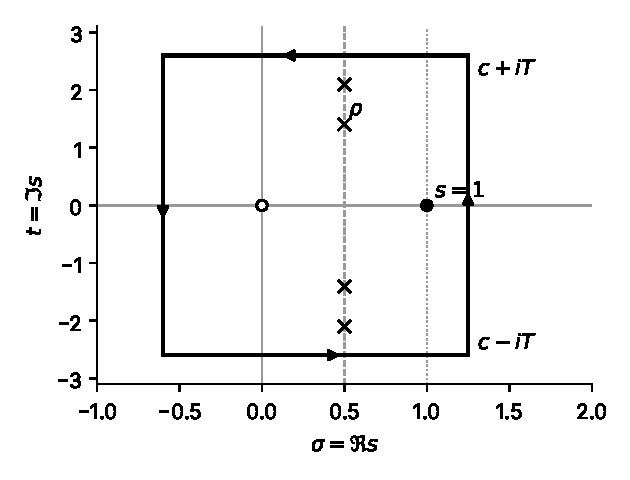
\includegraphics[width=0.62\textwidth]{figures/contour}
\caption{The contour used in the proof of \cref{lem:explicit}: the segment
$[c-iT,c+iT]$ is shifted to the left of the critical line, picking up the pole at
$s=1$ and the zeros $\rho$ with $\abs{\gamma}\le T$.}
\label{fig:contour}
\end{figure}

Subtracting \eqref{eq:explicit} at $x$ and $x+h$ and averaging over characters gives the
following.

\begin{theorem}\label{thm:short}
Let $\eps>0$ and $\theta> \frac{7}{12}+\eps$. For $x\ge x_0(\eps)$, $h=x^\theta$, and
$q\le (\log x)^{A}$,
\begin{equation}\label{eq:short}
\psi(x+h;q,a)-\psi(x;q,a) = \frac{h}{\varphi(q)}\left(1+\bigO{\exp\left(-c\frac{\log x}{(\log\log x)^{2/3}}\right)}\right)
\end{equation}
uniformly for $(a,q)=1$.
\end{theorem}

\begin{proof}
By orthogonality of characters,
\begin{align}
\psi(x+h;q,a)-\psi(x;q,a)
 &= \frac{1}{\varphi(q)}\sum_{\chi \bmod q}\bar\chi(a)\bigl(\psi(x+h,\chi)-\psi(x,\chi)\bigr)\label{eq:orth}\\
 &= \frac{h}{\varphi(q)} - \frac{1}{\varphi(q)}\sum_{\chi\bmod q}\bar\chi(a)
    \sum_{\abs{\gamma}\le T}\frac{(x+h)^{\rho}-x^{\rho}}{\rho} + \bigO{\frac{x\log^2 x}{T}}. \nonumber
\end{align}
Since $\abs{(x+h)^\rho-x^\rho}\le h x^{\beta-1}\abs{\rho}$, the double sum is at most
\[
 h\sum_{\chi}\sum_{\abs{\gamma}\le T} x^{\beta-1}
 \le h \int_0^1 x^{\sigma-1}\dd N(\sigma,T;q) \ll h\,(\log x)\max_{1/2\le\sigma\le1} x^{\sigma-1}N(\sigma,T;q),
\]
where $N(\sigma,T;q)$ counts zeros of all $\Lfun{\chi}$, $\chi\bmod q$, with
$\beta\ge\sigma$ and $\abs{\gamma}\le T$. Huxley's density estimate
$N(\sigma,T;q)\ll (qT)^{\frac{12}{5}(1-\sigma)}(\log qT)^{B}$ \cite[Ch.~12]{Ivic} and the
Vinogradov--Korobov zero-free region \cite{Korobov, Vinogradov} finish the proof with
$T=x^{1-\theta+\eps}$.
\end{proof}

\begin{remark}
The exponent $\frac{7}{12}$ is Huxley's \cite{Huxley}; any improvement in the density
hypothesis range transfers directly. The matrix
\[
\gamma=\begin{pmatrix} a & b\\ c & d\end{pmatrix}\in \mathrm{SL}_2(\Z),\qquad
\gamma\cdot z=\frac{az+b}{cz+d},
\]
plays no role here but is a reminder that the same method applies to Hecke $L$-functions,
for which the relevant maps fit in the diagram
\[
\begin{tikzcd}
\mathcal{S}_k(\Gamma_0(N)) \arrow[r, "\Lambda"] \arrow[d] & \mathcal{D} \arrow[d, "\mathcal{M}"] \\
\mathcal{S}_k(\Gamma_1(N)) \arrow[r] & \mathcal{H}
\end{tikzcd}
\]
of Mellin transforms.
\end{remark}

\begin{table}[ht]
\centering
\caption{Admissible exponents $\theta$ for \cref{thm:short} under various zero-density hypotheses.}
\label{tab:theta}
\begin{tabular}{lcc}
\hline
Density estimate & exponent $A(\sigma)$ & admissible $\theta$ \\
\hline
Ingham (1937) & $\frac{3}{2-\sigma}$ & $\theta>\frac58$ \\
Huxley (1972) & $\frac{12}{5}$ & $\theta>\frac{7}{12}$ \\
Density Hypothesis & $2$ & $\theta>\frac12$ \\
\hline
\end{tabular}
\end{table}

\section*{Acknowledgements}
We thank the referee for pointing out \cite{Titchmarsh}, and for the observation that
$\sum_{p\le x}\frac{\log p}{p}=\log x+O(1)$ suffices in \cref{sec:prelim}.

\bibliographystyle{amsplain}
\bibliography{refs}

\end{document}
